\section{Journey Options}
\label{sec:journey_options}
The Journey Options tab contains all of the settings necessary to define the spacecraft trajectory and the bodies it encounters along the way. An \ac{EMTG} mission requires at least one Journey, and each Journey contains an arrival and departure event. In early stages of mission design, a single Journey can model at low fidelity an entire mission including multiple flybys of Universe bodies. As mission design progresses, this low fidelity trajectory can be converted into multiple Journeys modeling different phases of the mission in higher accuracy. A single gravity assist may be modeled as a Journey from the \ac{SOI} crossing to periapse and another Journey from periapse to the next \ac{SOI} crossing. Chapter \ref{chap:conversion} discusses the tools \ac{EMTG} provides for converting low-fidelity missions into higher fidelity. Users should also reference Chapter \ref{chap:journey_boundaries} for more information on configuration of Journey arrival and departure events.

\noindent Figure \ref{fig:pyemtg_journey_options} show the default Journey Options tab in PyEMTG. There are many other Journey settings which are revealed based on other selections such as specifying the arrival state at a body. There are also multiple Journey settings which will override settings on other tabs that apply to the overall mission. 

    \begin{figure}[H]
        \centering
        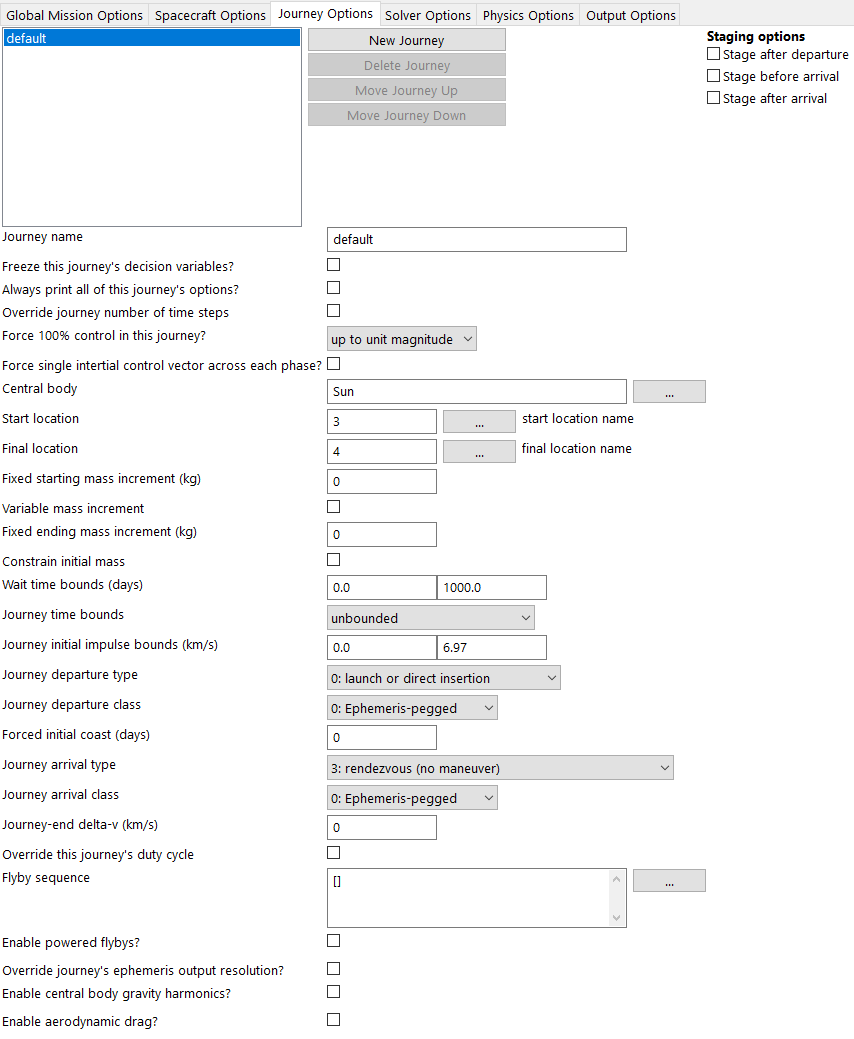
\includegraphics[width=0.9\textwidth]{../../shared_latex_inputs/images/pyemtg_journey_options_tab.png}
        \caption{EMTG Journey Options tab}
        \label{fig:pyemtg_journey_options}
    \end{figure}

\noindent In the upper left corner of the Journey Options tab is a set of buttons and a selector to manage the Journeys in the \ac{EMTG} options file. The rest of the options on the Journey Options tab correspond only to the currently selected Journey which will be highlighted in this window. The ``New Journey'' and ``Delete Journey'' buttons are used to create and remove Journeys from the \ac{EMTG} options file. The ``Move Journey Up'' and ``Move Journey Down'' buttons are used to change the order of the Journeys in the mission sequence. An \ac{EMTG} mission with several Journeys and a planetary flyby might look like the example in Figure \ref{fig:pyemtg_journey_manager}.

    \begin{figure}[H]
        \centering
        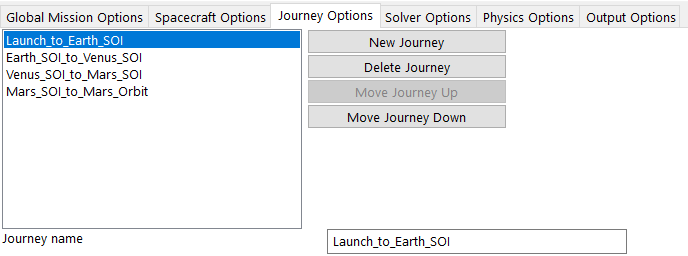
\includegraphics[width=0.7\textwidth]{../../shared_latex_inputs/images/pyemtg_journey_window.png}
        \caption{Journey Manager}
        \label{fig:pyemtg_journey_manager}
    \end{figure}

\subsection{Overall Journey Options}

    \begin{enumerate}

    \item \textbf{Journey Name:} The Journey name is used to distinguish the settings pertaining only to that Journey in the \ac{EMTG} options file and output files. Often these names specify the departure and arrival boundaries covered by the Journey.

        \begin{table}[H]
            \hspace{2cm}
            \begin{tabular}{ll}
            Data Type & \verb|string| \\
            Default Value & ``default'' \\
            \end{tabular}
        \end{table}

    
    \item \textbf{Freeze this journey's decision variables:} This options allows the user to hold the decision variables for the selected Journey constant when running \ac{EMTG}. The variables pertaining to any Journey with this setting selected in the \ac{EMTG} options file will not be changed by \ac{MBH} or \ac{SNOPT} at runtime. This can be used if only part of an \ac{EMTG} mission needs to be adjusted without interfering with other Journeys and can decrease \ac{EMTG}'s runtime.
        
        \begin{table}[H]
            \hspace{2cm}
            \begin{tabular}{ll}
            Data Type & \verb|bool| \\
            Allowed Values & true, false \\
            Default Value & false \\
            Units & NA
            \end{tabular}
        \end{table}

    \item \textbf{Always print all of this journey's options?:} This setting is similar to the ``Print only non-default options to .emtgopt file?'' setting on the Output Options tab (Section \ref{sec:output_options}). Selecting this option for a Journey will cause the \ac{EMTG} options file to show all options for the Journey even those which have not been changed from their default value. This setting overrides the ``Print only non-default options to .emtgopt file?'' setting on the Output Options tab.
        
        \begin{table}[H]
            \hspace{2cm}
            \begin{tabular}{ll}
            Data Type & \verb|bool| \\
            Allowed Values & true, false \\
            Default Value & false \\
            Units & NA
            \end{tabular}
        \end{table}

    \item \textbf{Override journey number of time steps?:} This setting allows the user to override the ``Number of time-steps'' setting on the Global Mission Options tab for the selected Journey. Selecting this option reveals and activates the ``Number of time steps'' setting in PyEMTG.
        
        \begin{figure}[H]
            \centering
            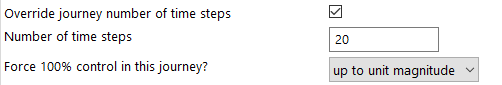
\includegraphics[width=0.7\textwidth]{../../shared_latex_inputs/images/pyemtg_journey_timesteps.png}
            \caption{Journey Time Steps}
            \label{fig:pyemtg_journey_timesteps}
        \end{figure}
    

        \begin{table}[H]
            \hspace{2cm}
            \begin{tabular}{ll}
            Data Type & \verb|bool| \\
            Allowed Values & true, false \\
            Default Value & false \\
            Units & NA
            \end{tabular}
        \end{table}

        \item \textbf{Number of time steps:} Override the number of time steps specified in the Global Options tab for this Journey only.

            \begin{table}[H]
                \hspace{2cm}
                \begin{tabular}{ll}
                Data Type & \verb|int| \\
                Allowed Values & 0 $<$ Integer $<$ $\infty$ \\
                Default Value & 20 \\
                Units & NA
                \end{tabular}
            \end{table}

    \item \textbf{Force 100\% control in this journey?:} A control 3-vector $\mathbf{u}$ is applied to each control segment in a low-thrust \ac{EMTG} Mission Type. The magnitude of $\mathbf{u}$ represents the duty cycle during that segment and is constrained to be $\leq 1$. This corresponds to the default option for this setting ``up to unit magnitude.'' The user may also select ``unit magnitude'' forcing the duty cycle to be 1.0 or ``zero magnitude'' forcing control to be off. This setting is only active when Journey Mission Type is \ac{MGALT}, \ac{FBLT}, \ac{PSBI}, or \ac{PSFB}.
    
        \begin{table}[H]
            \hspace{2cm}
            \begin{tabular}{lp{3cm}}
            Data Type & \verb|enum | \\
            Allowed Values & 
            \verb|0: up to unit magnitude,|\newline
            \verb|1: unit magnitude,|\newline 
            \verb|2: zero magnitude|  \\
            Default Value & 0 \\
            \end{tabular}
        \end{table}

    \item \textbf{Force single inertial control vector across each phase?:} This option forces \ac{EMTG} to point the control vector in a constant, inertial direction for the duration of the phase by forcing all control vectors to match each other.

        \begin{table}[H]
            \hspace{2cm}
            \begin{tabular}{ll}
            Data Type & \verb|bool| \\
            Allowed Values & true, false \\
            Default Value & false \\
            Units & NA
            \end{tabular}
        \end{table}


    \item \textbf{Central body:} Specifies the name of the \ac{EMTG} Universe file which contains the central body for this Journey as well as any other bodies necessary for this Journey.
    
        \begin{table}[H]
            \hspace{2cm}
            \begin{tabular}{ll}
            Data Type & \verb|string| \\
            Default Value & ``Sun'' \\
            \end{tabular}
        \end{table}


    \item \textbf{Start location:} Specifies the starting body for the Journey from the Universe file specified in the ``Central body'' option according to the number in the Universe file not the \ac{SPICE} ID.
    
        \begin{table}[H]
            \hspace{2cm}
            \begin{tabular}{ll}
            Data Type & \verb|int| \\
            Allowed Values & 1 $<$ Integer $\leq$ number of bodies in Universe file \\
            Default Value & 3 \\
            Units & NA
            \end{tabular}
        \end{table}

    \item \textbf{Final location:} Specifies the final body for the Journey from the Universe file specified in the ``Central body'' option according to the number in the Universe file not the \ac{SPICE} ID.
    
        \begin{table}[H]
            \hspace{2cm}
            \begin{tabular}{ll}
            Data Type & \verb|int| \\
            Allowed Values & 1 $<$ Integer $\leq$ number of bodies in Universe file \\
            Default Value & 4 \\
            Units & NA
            \end{tabular}
        \end{table}

    \item \textbf{Fixed starting mass increment (kg):} Increase the mass of the spacecraft at the start of this Journey by a fixed amount. Use a negative number to indicate a mass drop at the start of this Journey. 
    
        \begin{table}[H]
            \hspace{2cm}
            \begin{tabular}{ll}
            Data Type & \verb|double| \\
            Allowed Values & $-\infty$ $<$ Real $<$ $\infty$ \\
            Default Value & 0.0 \\
            Units & kg 
            \end{tabular}
        \end{table}


    \item \textbf{Variable mass increment (kg):} Selecting this option will convert the ``Fixed starting mass increment'' setting to  minimum and maximimum mass increment settings to bound the mass change at the start of the Journey.
        
        \begin{table}[H]
            \hspace{2cm}
            \begin{tabular}{ll}
            Data Type & \verb|bool| \\
            Allowed Values & true, false \\
            Default Value & false \\
            Units & NA
            \end{tabular}
        \end{table}

        \begin{figure}[H]
            \centering
            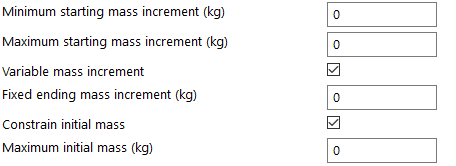
\includegraphics[width=0.7\textwidth]{../../shared_latex_inputs/images/pyemtg_journey_mass_increment.png}
            \caption{Journey Mass Increment Options}
            \label{fig:pyemtg_journey_mass_increment}
        \end{figure}

        
        \item \textbf{Minimum starting mass increment (kg):} Lower bound on Journey initial mass change. Use a negative number to indicate a mass drop at the start of this Journey. 
    
            \begin{table}[H]
                \hspace{2cm}
                \begin{tabular}{ll}
                Data Type & \verb|double| \\
                Allowed Values & $-\infty$ $<$ Real $<$ \verb|maximum starting mass increment| \\
                Default Value & 0.0 \\
                Units & kg 
                \end{tabular}
            \end{table}

        \item \textbf{Maximum starting mass increment (kg):} Upper bound on Journey initial mass change. Use a negative number to indicate a mass drop at the start of this Journey. 
    
            \begin{table}[H]
                \hspace{2cm}
                \begin{tabular}{ll}
                Data Type & \verb|double| \\
                Allowed Values & \verb|minimum starting mass increment| $<$ Real $<$ $\infty$ \\
                Default Value & 0.0 \\
                Units & kg 
                \end{tabular}
            \end{table}

    \item \textbf{Fixed ending mass increment (kg):} Increase the mass of the spacecraft at the end of this Journey by a fixed amount. Use a negative number to indicate a mass drop at the end of this Journey. 
    
        \begin{table}[H]
            \hspace{2cm}
            \begin{tabular}{ll}
            Data Type & \verb|double| \\
            Allowed Values & $-\infty$ $<$ Real $<$ $\infty$ \\
            Default Value & 0.0 \\
            Units & kg 
            \end{tabular}
        \end{table}
   

    \item \textbf{Constrain initial mass (kg):} Constrain the maximum value for the spacecraft mass at the start of this Journey. Reveals the ``Maximum initial mass'' setting.

        \begin{table}[H]
            \hspace{2cm}
            \begin{tabular}{ll}
            Data Type & \verb|bool| \\
            Allowed Values & true, false \\
            Default Value & false \\
            Units & NA
            \end{tabular}
        \end{table}

        \item \textbf{Maximum initial mass (kg):} Set the maximum value for the spacecraft mass at the start of this Journey.
        
            \begin{table}[H]
                \hspace{2cm}
                \begin{tabular}{ll}
                Data Type & \verb|double| \\
                Allowed Values & 0 $<$ Real $<$ $\infty$ \\
                Default Value & 0.0 \\
                Units & kg
                \end{tabular}
            \end{table}



    \item \textbf{Wait time bounds (days):} Bounds the time the spacecraft can remain at it's current body before departing on the next Journey. Can be used to remain in orbit around a body for a variable amount of time or delay launch from a body. 

        \begin{table}[H]
            \hspace{2cm}
            \begin{tabular}{ll}
            Data Type & \verb|double| \\
            Allowed Values & 0 $<$ Real $<$ $\infty$ \\
            Default Value & 0.0 and 1000.0\\
            Units & day
            \end{tabular}
        \end{table}

    \item \textbf{Journey time bounds:} Select whether to place bounds on the timespan of the Journey. Reveals additional settings depending on method chosen. Flight time refers to the sum of all phase time of flight variables and boundary event time widths in the Journey. Aggregate flight time refers to the sum of all phase flight time and boundary event time width variables up to and including the Journey. Arrival epoch computed by adding the launch epoch to the aggregate flight time.
    
        
        \begin{table}[H]
            \hspace{2cm}
            \begin{tabular}{lp{3cm}}
            Data Type & \verb| int| \\
            Allowed Values & \verb|0: unbounded, |\newline
            \verb|1: bounded flight time,|\newline 
            \verb|2: bounded arrival date,|\newline
            \verb|3: bounded aggregate flight time|  \\
            Default Value & 0 \\
            \end{tabular}
        \end{table}

            \item \textbf{Journey flight time bounds (days):} Set bounds on the flight time of the Journey in days. Revealed when ``Journey time bounds'' is set to ``bounded flight time'' or ``bounded aggregate flight time.''
            
                \begin{table}[H]
                    \hspace{2cm}
                    \begin{tabular}{ll}
                    Data Type & \verb|double| \\
                    Allowed Values & 0 $<$ Real $<$ $\infty$ \\
                    Default Value & 0.0 and 1000.0\\
                    Units & day
                    \end{tabular}
                \end{table}

            \item \textbf{Journey arrival date bounds:} Set bounds on the arrival date of the Journey in days. Revealed when ``Journey time bounds'' is set to ``bounded arrival date.'' Enter a date in MJD2000 or select date using the calendars revealed in PyEMTG.           

                \begin{table}[H]
                    \hspace{2cm}
                    \begin{tabular}{ll}
                    Data Type & \verb|double| \\
                    Allowed Values & 0 $<$ Real $<$ $\infty$ \\
                    Default Value & 51544.5 and 60000.0\\
                    Units & days since MJD2000 epoch
                    \end{tabular}
                \end{table}

                \begin{figure}[H]
                    \centering
                    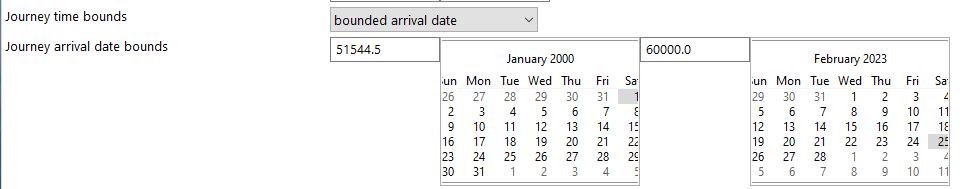
\includegraphics[width=1.0\textwidth]{../../shared_latex_inputs/images/pyemtg_journey_bounded_arrival.png}
                    \caption{Journey bounded arrival date}
                \end{figure}

    \end{enumerate}

\subsection{Journey Departure Options}
    \begin{enumerate}
    \item \textbf{Journey initial impulse bounds (km/s):} Set bounds on the initial impulsive velocity change occurring at the departure phase of the Journey. Only applicable when ``Journey departure type'' is ``launch or direct insertion,'' or ``depart parking orbit.''
    
        \begin{table}[H]
            \hspace{2cm}
            \begin{tabular}{ll}
            Data Type & \verb|double| \\
            Allowed Values & 0 $<$ Real $<$ $\infty$ \\
            Default Value & 0.0 and 6.97\\
            Units & km/s
            \end{tabular}
        \end{table}

    \item \textbf{Journey departure type:} Set the departure type for the Journey. See Chapter \ref{chap:journey_boundaries} for discussion on departure type and departure class combinations. Reveals additional options depending on setting.
    
        \begin{table}[H]
            \hspace{2cm}
            \begin{tabular}{lp{3cm}}
            Data Type & \verb| (DepartureType) enum| \\
            Allowed Values & \verb|0: launch or direct insertion,|\newline
            \verb|1: depart parking orbit,| \newline 
            \verb|2: free direct departure, |\newline
            \verb|3: flyby| \newline 
            \verb|4: flyby with fixed v-infinity-out,| \newline 
            \verb|5: spiral out from circular orbit,| \newline
            \verb|6: zero-turn flyby (for small bodies)| \\
            Default Value & \verb|0: launch or direct insertion |\\
            \end{tabular}
        \end{table}

    \item \textbf{Journey departure class:} Set the departure class for the Journey. See Chapter \ref{chap:journey_boundaries} for discussion on departure type and departure class combinations.
    
        \begin{table}[H]
            \hspace{2cm}
            \begin{tabular}{lp{3cm}}
            Data Type & \verb| (BoundaryClass) enum| \\
            Allowed Values & \verb|0: Ephemeris-pegged, |\newline
            \verb|1: Free point,| \newline 
            \verb|2: Ephemeris-referenced,|\newline 
            \verb|3: Periapse| \\
            Default Value & \verb|0: Ephemeris-pegged|\\
            \end{tabular}
        \end{table}

    \item \textbf{Forced initial coast (days):} Forces the spacecraft to coast from it's initial state for some number of days before performing any maneuvers. Similar to ``forced post-flyby coast duration'' on the Global Mission Options tab (Section \ref{sec:global_options}). 
        
        \begin{table}[H]
            \hspace{2cm}
            \begin{tabular}{ll}
            Data Type & \verb|double| \\
            Allowed Values & 0 $<$ Real $<$ $\infty$ \\
            Default Value & 0 \\
            Units & days 
            \end{tabular}
        \end{table}

    \item \textbf{Orbital radius for beginning of escape spiral (km):} Revealed when ``Journey departure type'' is set to ``spiral out from circular orbit.'' Sets the starting circular orbit radius to begin the low-thrust spiral escape from the departure body.
        
        \begin{table}[H]
            \hspace{2cm}
            \begin{tabular}{ll}
            Data Type & \verb|double| \\
            Allowed Values & 0 $<$ Real $<$ $\infty$ \\
            Default Value & 0 \\
            Units & km 
            \end{tabular}
        \end{table}

    \item \textbf{Orbital radius for end of escape spiral (km):} Revealed when ``Journey departure type'' is set to ``spiral out from circular orbit.'' Sets the final circular orbit radius to finish the low-thrust spiral escape from the departure body.
        
        \begin{table}[H]
            \hspace{2cm}
            \begin{tabular}{ll}
            Data Type & \verb|double| \\
            Allowed Values & 0 $<$ Real $<$ $\infty$ \\
            Default Value & 0 \\
            Units & km 
            \end{tabular}
        \end{table}

    \end{enumerate}


\subsection{Journey Arrival Options}

    \begin{enumerate}


    \item \textbf{Journey arrival type:} Set the arrival type for the Journey. See Chapter \ref{chap:journey_boundaries} for discussion on arrival type and arrival class combinations. Reveals additional options depending on setting.

        \begin{table}[H]
            \hspace{2cm}
            \begin{tabular}{lp{3cm}}
            Data Type & \verb| (ArrivalType) enum| \\
            Allowed Values & \verb|0: insertion into parking orbit (use chemical Isp),| \newline 
            \verb|1: rendezvous (with chemical maneuver),| \newline 
            \verb|2: intercept with bounded V_infinity,| \newline 
            \verb|3: rendezvous (no maneuver)| \newline 
            \verb|4: match final v-infinity vector (with chemical maneuver),| \newline 
            \verb|5: match final v-infinity vector (no maneuver),| \newline
            \verb|6: capture spiral, |\newline
            \verb|7: momentum transfer|\\
            Default Value & \verb|3: launch or direct insertion |\\
            \end{tabular}
        \end{table}

    \item \textbf{Journey arrival class:} Set the arrival class for the Journey. See Chapter \ref{chap:journey_boundaries} for discussion on arrival type and arrival class combinations. Reveals additional options depending on setting.
        \begin{table}[H]
            \hspace{2cm}
            \begin{tabular}{lp{3cm}}
            Data Type & \verb| (BoundaryClass) enum| \\
            Allowed Values & \verb|0: Ephemeris-pegged, 1: Free point,| \newline 
            \verb|2: Ephemeris-referenced, 3: Periapse|\\
            Default Value & \verb|0: Ephemeris-pegged|\\
            \end{tabular}
        \end{table}

    \item \textbf{Impact momentum enhancement factor (beta):} Set a scale factor that encompasses the plasticity of the impact, the crater formation, and the ejecta released by the impact for the special case where the spacecraft collides with the destination body and transfers momentum to it. See the \ac{EMTG} Software Design Document, Section 13.5.2.7 for more information.
        
        \begin{table}[H]
            \hspace{2cm}
            \begin{tabular}{ll}
            Data Type & \verb|double| \\
            Allowed Values & 0 $<$ Real $<$ $\infty$ \\
            Default Value & 1 \\
            Units & NA 
            \end{tabular}
        \end{table}


    \item \textbf{Orbital radius for beginning of capture spiral (km):} Revealed when ``Journey arrival type'' is set to ``capture spiral.'' Sets the starting circular orbit radius to begin the low-thrust capture spiral at the arrival body.
    
        \begin{table}[H]
            \hspace{2cm}
            \begin{tabular}{ll}
            Data Type & \verb|double| \\
            Allowed Values & 0 $<$ Real $<$ $\infty$ \\
            Default Value & 6678\\
            Units & km
            \end{tabular}
        \end{table}

    \item \textbf{Orbital radius for end of capture spiral (km):} Revealed when ``Journey arrival type'' is set to ``capture spiral.'' Sets the final circular orbit radius to end the low-thrust capture spiral at the arrival body.
    
        \begin{table}[H]
            \hspace{2cm}
            \begin{tabular}{ll}
            Data Type & \verb|double| \\
            Allowed Values & 0 $<$ Real $<$ $\infty$ \\
            Default Value & 6678\\
            Units & km
            \end{tabular}
        \end{table}
%#!! stopped here.
    \item \textbf{Journey-end delta-v (km/s):} Reduce the propellant mass of the spacecraft at the end of the Journey. In order to account for maneuvers that will be performed after arrival at the target body. This could be expressed as a fixed mass drop, but journey end delta-v allows the user to define a delta-v and apply it against the spacecraft mass at the end of the journey, using the appropriate spacecraft stage monopropellant system.
        
        \begin{table}[H]
            \hspace{2cm}
            \begin{tabular}{ll}
            Data Type & \verb|double| \\
            Allowed Values & 0 $<$ Real $<$ $\infty$ \\
            Default Value & 0 \\
            Units & km/s 
            \end{tabular}
        \end{table}

    \end{enumerate}

\subsection{Perturbations and Other Options}
    \label{sec:journey_perturbations}
    \begin{enumerate}    
    
    \item \textbf{Override this journey's duty cycle:} Override the spacecraft duty cycle specified on the Spacecraft Options tab for this Journey only. Reveals the Journey duty cycle setting.

    \begin{table}[H]
        \hspace{2cm}
        \begin{tabular}{ll}
        Data Type & \verb|bool| \\
        Allowed Values & true, false \\
        Default Value & false \\
        Units & NA
        \end{tabular}
    \end{table}

    \item \textbf{Journey duty cycle:} Set the spacecraft duty cycle for this Journey only overriding the setting specified on the Spacecraft Options tab.

        \begin{table}[H]
            \hspace{2cm}
            \begin{tabular}{ll}
            Data Type & \verb|double| \\
            Allowed Values & 0 $<$ Real $<$ $\infty$ \\
            Default Value & 1\\
            Units & NA
            \end{tabular}
        \end{table}

    \item \textbf{Flyby sequence:} Specify a sequence of bodies the spacecraft should flyby during this Journey modeled using patched conics. The integers listed should correspond to the body number in the ``menu of bodies'' section of the Universe file specified for this Journey.

        \begin{table}[H]
            \hspace{2cm}
            \begin{tabular}{ll}
            Data Type & \verb|std::vector<int, n>| \\
            Allowed Values & Integers from the set of bodies in Universe file \\
            Default Value & [ ] \\
            Units & NA
            \end{tabular}
        \end{table}

    \item \textbf{Enable powered flybys?:} Allow delta-v changes to occur during body flybys.%#?? is this only for patched conics?

        \begin{table}[H]
            \hspace{2cm}
            \begin{tabular}{ll}
            Data Type & \verb|bool| \\
            Allowed Values & true, false \\
            Default Value & false \\
            Units & NA
            \end{tabular}
        \end{table}

    \item \textbf{Perturbation\_bodies:} Select bodies by number in the Universe file for this Journey that will contribute to third body gravitational perturbing forces on the spacecraft. Revealed when the user selects ``Enable third body'' on the Physics Options tab (see Sec:\ref{sec:physics_options}).
    
        \begin{table}[H]
            \hspace{2cm}
            \begin{tabular}{ll}
            Data Type & \verb|std::vector<int, n>| \\
            Allowed Values & Integers from the set of bodies in Universe file \\
            Default Value & [ ] \\
            Units & NA
            \end{tabular}
        \end{table}

    \item \textbf{Override journey's ephemeris output resolution?:} Override the forward propagated epehemeris resolution set in the Output Options tab. This setting has no effect if the ``Generate forward-integrated ephemeris'' setting is not active.

        \begin{table}[H]
            \hspace{2cm}
            \begin{tabular}{ll}
            Data Type & \verb|bool| \\
            Allowed Values & true, false \\
            Default Value & false \\
            Units & NA
            \end{tabular}
        \end{table}

        \item \textbf{Ephemeris output resolution (seconds):} Set the forward propagated ephemeris resolution for this Journey only.

            \begin{table}[H]
                \hspace{2cm}
                \begin{tabular}{ll}
                Data Type & \verb|double| \\
                Allowed Values & 1e-3 $<$ Real $<$ $\infty$ \\
                Default Value & 1\\
                Units & seconds
                \end{tabular}
            \end{table}

    \item \textbf{Enable central body gravity harmonics?:} Activate spherical harmonics gravity perturbations for the central body of this Journey. This setting requires an appropriate propagator and Mission Type combination (see Chapter \ref{chap:force_model_prop}) and a gravity file for the central body with a {\tt .grv} extension. 

            \begin{table}[H]
                \hspace{2cm}
                \begin{tabular}{ll}
                Data Type & \verb|bool| \\
                Allowed Values & true, false \\
                Default Value & false \\
                Units & NA
                \end{tabular}
            \end{table}

            \item \textbf{Central body gravity data file:} Path to the gravity file for the central body of the Journey specifying the spherical harmonics information. See Section \ref{sec:force_model_spherical_harmonics} for details on the expected structure of the {\tt .grv} file.

                \begin{table}[H]
                    \hspace{2cm}
                    \begin{tabular}{ll}
                    Data Type & \verb|string| \\
                    Default Value & ``DoesNotExist.grv'' \\
                    \end{tabular}
                \end{table}

            \item \textbf{Central body maximum degree:} Set the maximum degree for spherical harmonics perturbations. Information up to this degree must be specified in the gravity file.

                \begin{table}[H]
                    \hspace{2cm}
                    \begin{tabular}{ll}
                    Data Type & \verb|int| \\
                    Allowed Values & 0 $<$ Integer $<$ $\infty$ \\
                    Default Value & 2 \\             
                    \end{tabular}
                \end{table}
                
                \item \textbf{Central body maximum order:} Set the maximum order for spherical harmonics perturbations. Information up to this order must be specified in the gravity file.

                \begin{table}[H]
                    \hspace{2cm}
                    \begin{tabular}{ll}
                    Data Type & \verb|int| \\
                    Allowed Values & 0 $<$ Integer $<$ $\infty$ \\
                    Default Value & 0 \\
                    \end{tabular}
                \end{table}
    

     
    \item \textbf{Enable aerodynamic drag?:} Enable aerodynamic drag acceleration modeling due to the central body during this Journey. Requires a {\tt .emtg\_densityopt} options file defining density information. See Section \ref{sec:force_model_drag} for details on the expected structure of the {\tt .emtg\_densityopt} file.

        \begin{table}[H]
            \hspace{2cm}
            \begin{tabular}{ll}
            Data Type & \verb|bool| \\
            Allowed Values & true, false \\
            Default Value & false \\
            Units & NA
            \end{tabular}
        \end{table}

    \item \textbf{Spacecraft drag area (m\^{}2):} Set spacecraft area used to aerodynamic drag. Only active when ``Enable aerodynamic drag'' is selected.

        \begin{table}[H]
            \hspace{2cm}
            \begin{tabular}{ll}
            Data Type & \verb|double| \\
            Allowed Values & 0 $<$ Real $<$ $\infty$ \\
            Default Value & 70 \\
            Units & $m^2$
            \end{tabular}
        \end{table}

    \item \textbf{Spacecraft drag coefficient:} Set spacecraft drag coefficient used to aerodynamic drag. Only active when ``Enable aerodynamic drag'' is selected.

        \begin{table}[H]
            \hspace{2cm}
            \begin{tabular}{ll}
            Data Type & \verb|double| \\
            Allowed Values & 0 $<$ Real $<$ $\infty$ \\
            Default Value & 2.2 \\
            Units & NA
            \end{tabular}
        \end{table}

    \item \textbf{Atmospheric density model:} Select the atmospheric density model to use. Only Exponential is currently available. Only active when ``Enable aerodynamic drag'' is selected.

        \begin{table}[H]
            \hspace{2cm}
            \begin{tabular}{lp{3cm}}
            Data Type & \verb|str| \\
            Allowed Values & \verb|Exponential|\\
            Default Value & \verb|Exponential|\\
            \end{tabular}
        \end{table}

    \item \textbf{Atmospheric density model data file:} Specifies the atmospheric density model file, a {\tt .emtg\_densityopt} file containing the altitude versus density information used in drag calculations. See Section \ref{sec:force_model_drag} for details on the expected structure of the {\tt .emtg\_densityopt} file. Only active when ``Enable aerodynamic drag'' is selected.

            \begin{table}[H]
                \hspace{2cm}
                \begin{tabular}{ll}
                Data Type & \verb|string| \\
                Default Value & ``DoesNotExist.emtg\_densityopt'' \\
                \end{tabular}
            \end{table}
    \end{enumerate}

\subsection{Departure and Arrival Elements}
\label{sec:journey_dep_arrive_elements}
Selecting Free-point on either the Departure or Arrival Class will reveal new options allowing the user to specify specific state elements expressed in cartesian, spherical, orbital elements, or b-plane representations. State elements may be fixed or allowed to vary within user-specified bounds.

    \begin{figure}[H]
        \centering
        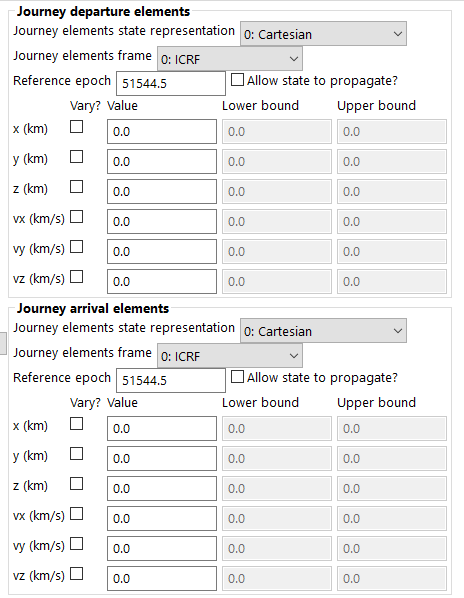
\includegraphics{../../shared_latex_inputs/images/pyemtg_journey_deparr_elements.png}
        \caption{EMTG Journey Arrival and Depature Elements}
        \label{fig:pyemtg_journey_deparr_elements}
    \end{figure}




\begin{enumerate}
    \item \textbf{Journey elements state representation:} Select how the Journey Arrival/Departure state will be represented when the Boundary Class is set to Free Point.
    
    
    \begin{table}[H]
        \hspace{2cm}
        \begin{tabular}{lp{3cm}}
        Data Type & \verb| (StateRepresentation) enum| \\ 
        Allowed Values & \verb|0: Cartesian,| \newline 
            \verb|1: SphericalRADEC,| \newline 
            \verb|2: SphericalAZFPA,| \newline 
            \verb|3: COE, 4: MEE,| \newline 
            \verb|5: IncomingBplane,| \newline
            \verb|6: OutgoingBplane,|\newline
            \verb|7: IncomingBplaneRpTA|\newline
            \verb|8: OutgoingBplaneRpTA,| \\
        Default Value & \verb|0: Cartesian, | \\
        \end{tabular}
    \end{table}

    \item \textbf{Journey elements frame:} Select the reference frame for the Journey Arrival/Departure state when the Boundary Class is set to Free Point.

        \begin{table}[H]
            \hspace{2cm}
            \begin{tabular}{lp{3cm}}
            Data Type & \verb| (ReferenceFrame) enum| \\
            Allowed Values & \verb|0: ICRF,| \newline 
            \verb|1: J2000_BCI,| \newline 
            \verb|2: J2000_BCF,| \newline 
            \verb|3: TrueOfDate_BCI| \newline 
            \verb|4: TrueOfDate_BCF,| \newline 
            \verb|5: PrincipleAxes,| \newline
            \verb|6: Topocentric, |\newline
            \verb|7: Polar|\newline
            \verb|8: SAM|\newline
            \verb|9: Object Referenced|\\
            Default Value & \verb|0: ICRF |\\
            \end{tabular}
        \end{table}

    \item \textbf{Reference epoch:} Epoch for the specified Journey arrival/departure state in MJD2000.
    
        \begin{table}[H]
            \hspace{2cm}
            \begin{tabular}{ll}
            Data Type & \verb|double| \\
            Allowed Values & $0$ $<$ Real $<$ $\infty$ \\
            Default Value & 51544.5\\
            Units & days since MJD2000 epoch
            \end{tabular}
        \end{table}

    \item \textbf{Allow state to propagate?:} Selecting this option allows the state to propagate forward or backward from the specified epoch. Otherwise the Free point represents a fixed waypoint.

        \begin{table}[H]
            \hspace{2cm}
            \begin{tabular}{ll}
            Data Type & \verb|bool| \\
            Allowed Values & true, false \\
            Default Value & false \\
            Units & NA
            \end{tabular}
        \end{table}

    \item \textbf{Journey Arrival/Departure State:} Specify the six state components for the selected state representation as well as whether they can vary and their bounds. If the user chooses to fix any of these values, they are still variables but their bounds are ±1.0e-13, so the solver cannot move them.
    
        \begin{table}[H]
            \hspace{2cm}
            \begin{tabular}{ll}
            Data Type & \verb|double| \\
            Allowed Values & $-\infty$ $<$ Real $<$ $\infty$ \\
            Default Value & 0.0\\
            Units & various
            \end{tabular}
        \end{table}

\end{enumerate}

\subsection{Journey Staging Options}

    \begin{enumerate}

        \item \textbf{Stage after departure:} Stage the spacecraft according to the spacecraft configuration file immediately following departure. See Chapter \ref{chap:config_files}.

            \begin{table}[H]
                \hspace{2cm}
                \begin{tabular}{ll}
                Data Type & \verb|bool| \\
                Allowed Values & true, false \\
                Default Value & false \\
                Units & NA
                \end{tabular}
            \end{table}

        \item \textbf{Stage before arrival:} Stage the spacecraft according to the spacecraft configuration file immediately before arrival. See Chapter \ref{chap:config_files}.

            \begin{table}[H]
                \hspace{2cm}
                \begin{tabular}{ll}
                Data Type & \verb|bool| \\
                Allowed Values & true, false \\
                Default Value & false \\
                Units & NA
                \end{tabular}
            \end{table}

        \item \textbf{Stage after arrival:} Stage the spacecraft according to the spacecraft configuration file immediately following arrival. See Chapter \ref{chap:config_files}.

            \begin{table}[H]
                \hspace{2cm}
                \begin{tabular}{ll}
                Data Type & \verb|bool| \\
                Allowed Values & true, false \\
                Default Value & false \\
                Units & NA
                \end{tabular}
            \end{table}

    \end{enumerate}



